\chapter{Rufzeichen}

\section{Schweizer Rufzeichen HBn und HEn}
\begin{tabular}{l p{9cm}}
\bfseries Rufzeichen & \bfseries Verwendung \\ \toprule \arrayrulecolor{rowsep}
HB9 & Normales Präfix für lizenzierte Amateurfunker in der Schweiz. \\ \midrule
HB9x(x) & \textit{Oldtimer} der 60er-Jahre (z. B. Rudolf Stuber mit HB9T) oder \textit{Klubstationen}. \\ \midrule
HB0 & Amateurfunker aus Lichtenstein. (Internet: TLD .li, bei Autokennzeichen FL) \\ \midrule
HB4 & Station der Schweizer Armee. \\ \midrule
HB3 & Einsteigerlizenz \\ \midrule
HB2 & Dieses Präfix wurde 2000 und 2003 verwendet, als Kantone ihr 200-Jahre-Jubiläum feierten. \\ \midrule
HB5 & Nur wenige Stationen \\ \midrule
HE7 & Spezielles Präfix \\ \midrule
HE9xxx & Rufzeichen für Zuhörer. Sie wurden von der PTT vergeben. \\ \midrule
\end{tabular}

{
\newcommand{\rz}[1]{\texttt{#1}}

\section{Rufzeichenbildung der verschiedenen Funkdienste nach ITU}
\subsection{Allgemein}
Zur Bildung von Rufzeichen können die 26 Buchstaben des Alphabets und, in den nachstehend angegebenen Fällen, auch die Ziffern verwendet werden. Ausgenommen sind Buchstaben mit Akzent.

Die beiden ersten Zeichen oder, in bestimmten Fällen, das erste Zeichen eines Rufzeichens dienen bzw. dient der Kennzeichnung der Nationalität. Bei den mit B, F, G, I, K, M, N, R und W beginnenden Rufzeichen wird nur das erste Zeichen für die Kennzeichnung der Nationalität benötigt.

In der folgenden Tabelle gilt \texttt{a}: Buchstabe, \texttt{9}: Zahl, \texttt{x}: Buchstabe oder Zahl.

\vspace{1em}
\noindent
\begin{tabular}{ll}
\bfseries Stationsart & \bfseries Rufzeichen \\ \toprule \arrayrulecolor{rowsep}
Land-/Fixstationen    & \rz{xxa}, \rz{xxa9}, \rz{xxa99}, \rz{xxa999} \\ \midrule
Mobile Landstationen  & \rz{xa9999}, \rz{xxa9999}, \rz{xxaa9999} \\ \midrule
Mobiler Seefunk       & \rz{xxaa}, \rz{xxaa9}, \rz{xxaa99}, \rz{xa999}, \rz{xxa9999} \\ \midrule
Mobiler Flugfunk      & \rz{xxaaa}, \rz{xaaaa}, \rz{x9999} \\ \midrule
Amateurfunk           & \rz{xx9a}, \rz{xx9xa}, \rz{xx9xxa}, \rz{xx9xxxa}, \rz{a9a}, \rz{a9xa}, \rz{a9xxa}, \rz{a9xxxa} \\ \midrule
Weltraumfunkdienste   & \rz{xx99}, \rz{xx999} (Ziffer nach Buchstabe darf nicht 0 oder 1 sein) \\ \midrule
\end{tabular}

\subsection{Flugfunk}
Abgekürzte Rufzeichen werden durch das erste und die beiden letzten Zeichen des Rufzeichens gebildet. Beispiele:
\begin{itemize}
 \item \rz{HB-IMJ} abgekürzt: \rz{H-MJ}
 \item \rz{HB-ISB} abgekürzt: \rz{H-SB}
\end{itemize}
Rufzeichen werden abgekürzt, sobald das Flugzeug bzw. der Helikopter von der Gegenstelle (zum Beispiel dem Tower) identifiziert ist. 

Flugzeuge können auch nach der Fluggesellschaft benannt werden, mit nachfolgender Flugnummer. Abgekürzte Rufzeichen sind hier nicht zulässig. Beispiele:
\begin{itemize}
 \item \rz{SWISS 100}
 \item \rz{SPEEDBIRD 2342}
\end{itemize}

Rettungsgerätefunkstellen von Flugzeugen bestehen aus dem vollständigen Rufzeichen des Flugzeuges (zivile Immatrikulation) und nur einer Ziffer ausser 0 oder 1. Beispiel: 
\rz{HB-XAD 3}

Bodenfunkstellen werden mit dem Namen des Flughafens oder der geografische Name des Ortes, dem nötigenfalls ein geeignetes Wort folgt, das den Zweck der Bodenfunkstelle angibt, bezeichnet. Beispiele:
\begin{itemize}
 \item \rz{ZURICH TOWER}
 \item \rz{ZURICH APPROACH}
\end{itemize}

Der Dienst wird folgendermassen bezeichnet:

\begin{longtabu}{ll}
\bfseries Name & \bfseries Beschreibung \\ \toprule 
\endhead \arrayrulecolor{rowsep}
\rz{TOWER} & Platzverkehrsleitung \\ \midrule
\rz{GROUND} & Bodenverkehrsleitung \\ \midrule
\rz{RADIO} & Bodenfunkstelle \\ \midrule
\rz{APRON} & Vorfeldkontrolle \\ \midrule
\rz{RADAR} & Radar (allgemein) \\ \midrule
\rz{CONTROL} & Bezirksverkehrsleitung (ohne Radar) \\ \midrule
\rz{APPROACH} & Anflugleitung (ohne Radar) \\ \midrule
\rz{ARRIVAL} & Anflugleitung (mit Radar) \\ \midrule
\rz{PRECISION} & Präzisionsanflugradar \\ \midrule
\rz{DEPARTURE} & Abflugleitung (mit Radar) \\ \midrule
\rz{DELIVERY} & ATC\footnote{Air Traffic Control, Flugverkehrsleitung}-Freigaben \\ \midrule
\rz{DELTA/TERMINAL} & ATC-Freigaben CH (Lufträume D/C\footnote{Lufträume D und C dürfen ohne Bewilligung nicht betreten werden. Für den Luftraum C ist jeweils eine separate Bewilligung notwendig, auch wenn man sich bereits im Flugraum D befindet.}) \\ \midrule
\rz{INFORMATION} & Fluginformationsdienst \\ \midrule
\rz{AERODROME} & Flugplatzinformationsdienst (AFIS) \\ \midrule
\rz{DISPATCH} & Flugdienstberatungsstelle \\ \midrule
\rz{HOMER} & Peilstelle \\ \midrule
\end{longtabu}

\subsection{Genauere Zuordnung der Rufzeichen}
In der Schweiz werden Rufzeichen heutzutage der Reihe nach vergeben, in einigen grösseren Ländern jedoch nach Region: So wird ersichtlich, wo der Funker die Lizenz bekommen hat. Dies ist beispielsweise in England, Russland und Kanada der Fall. In Russland gibt die Zahl die Region an und der Buchstabe danach das \textit{Oblast} (Verwaltungsbezirk).\footnote{Genaurere Informationen dazu auf der Englischen \href{http://en.wikipedia.org/wiki/Amateur\_radio\_call\_signs\_of\_Russia}{Wikipedia:Amateur\_radio\_call\_signs\_of\_Russia}.}

\begin{figure}[h!]
 \centering
 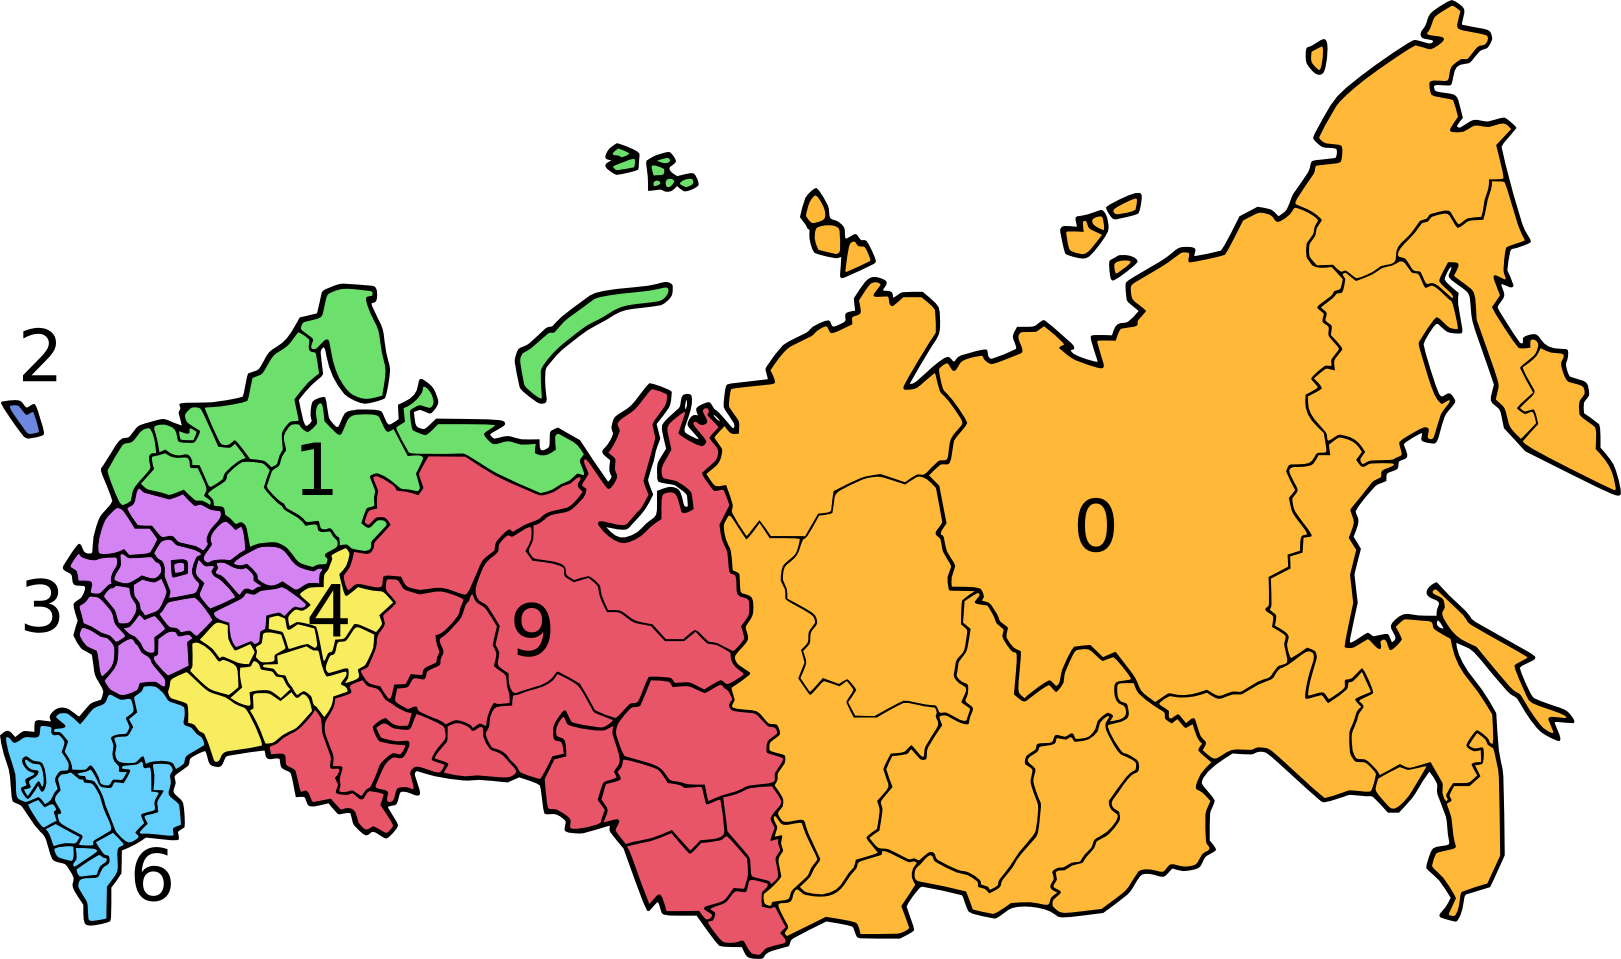
\includegraphics[width=8cm]{./png/Russia-amateur-callsign-districts.png}
 % Russia-amateur-callsign-districts.png: 1621x959 pixel, 90dpi, 45.77x27.08 cm, bb=0 0 1297 767
 \caption{Grobe Einteilung der Amateurfunk-Rufzeichen in Russland. \imgsrc{\href{http://en.wikipedia.org/wiki/File:Russia_amateur_callsign_districts.svg}{Chris Rovulo}, GFDL 1.2, cc-by-sa 3.0}}
 \label{fig:callsignsRU}
\end{figure}

\begin{figure}[h!]
 \centering
 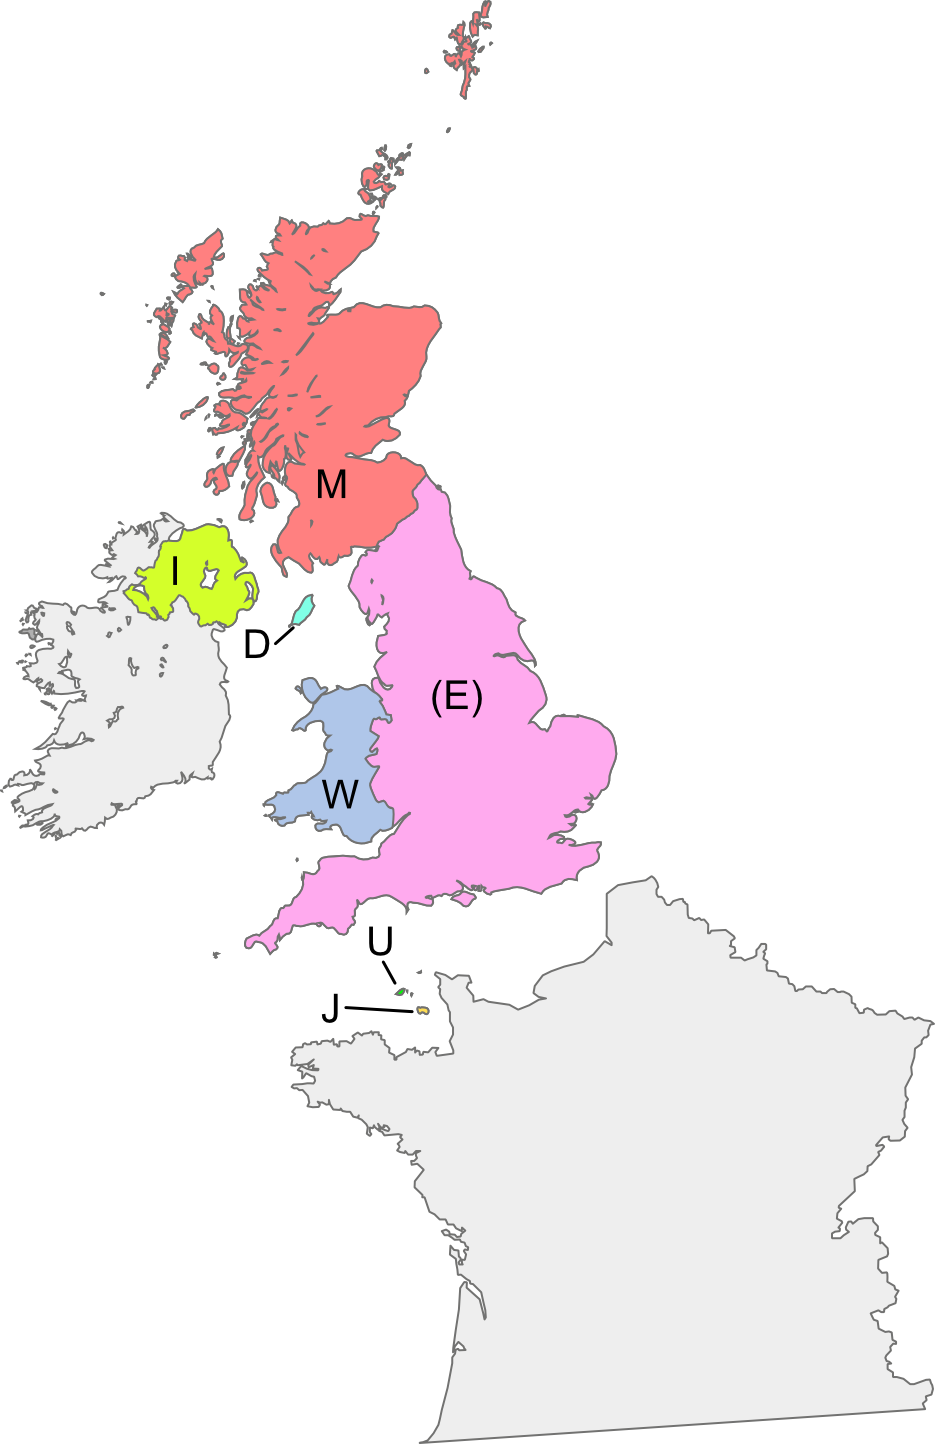
\includegraphics[height=6cm]{./png/UK-amateur-radio-regional-locators.png}
 % UK-amateur-radio-regional-locators.png: 935x1444 pixel, 90dpi, 26.39x40.76 cm, bb=0 0 748 1155
 \caption{Amateur-Rufzeichen in den UK. \imgsrc{\href{http://en.wikipedia.org/wiki/File:UK_amateur_radio_regional_locators.svg}{Adambro}, PD}}
 \label{fig:callsignsUK}
\end{figure}



\section{Kurzbeschrieb der Funkdienste}
\paragraph{Fixed Service} Dienst zwischen zwei festgelegten fixen Bodenstationen
\paragraph{Fixed — Satellite Service} Dienst zwischen Erdstation, wenn einer oder mehrere Satelliten benutzt werden
\paragraph{Mobile Service} Dienst zwischen mobilen und Landstationen oder zwischen mobilen Stationen
\paragraph{Mobile — Satellite Service} Dienst zwischen mobilen Erdstationen und einer oder mehreren Weltraumstationen oder zwischen Welt­raum­stationen
\paragraph{Maritime Mobile Service} Ein mobiler Dienst zwischen Küstenstationen und Schiffstationen oder zwischen Schiff­sta­tio­nen
\paragraph{Maritime Mobile — Satellite Service} Ein mobiler satellitengestützer Dienst, bei welchem sich mobile Erdstationen auf Schiffen befinden
\paragraph{Port-Operations Service} Ein mobiler Seefunk-Dienst in einem oder in der Nähe eines Hafens, zwischen Küstenstationen und Schiffstationen oder zwischen Schiffstationen
\paragraph{Aeronautical Mobile Service} Ein mobiler Dienst zwischen Flugbodenstationen und Luftfahrzeugen oder zwischen Luftfahr­zeugen
\paragraph{Broadcasting Service} Ein Dienst, bei welchem die Aussendungen für den direkten Empfang bei der Bevölkerung vorgesehen sind
\paragraph{Radio Amateur Service} Amateurfunk, wird von privaten Personen als Hobby betrieben







}